
\chapter{Gardez les pieds sur Terre}
Plutôt que de placer notre terrain comme une simple entité dans la scène (ce qui serait très laborieux), Ogre propose de passer par une classe Terrain pour la gestion des terrains dans la scène.

Le terrain n'est généralement pas seul et le ciel joue un rôle important pour le réalisme de la scène. Là encore, quelques outils bienvenus offrent différentes solutions pour obtenir un résultat convaincant.



\section{Créer un terrain}


\subsection{Préparation}

Avant de commencer, il va falloir modifier un peu notre projet avec de nouvelles dépendances pour que les terrains soient utilisables.

Il faut ajouter un fichier en-tête dans notre classe :

\begin{lstlisting}[caption={Ajout du fichier d'entête pour la gestion des terrains}]
#include <Ogre/Terrain/OgreTerrain.h>
\end{lstlisting}

Pour la prise en compte des lib
\begin{itemize}
\item OgreTerrain.dll
\item OgrePaging.dll
\end{itemize}

il va nous ajouter les lignes suivantes au fichier CMakeList.txt:

\begin{lstlisting}[caption={Modification de CMakeLists.txt pour l'inclusion des lib Terrain et Paging}]
#Inclusion de la lib libOgreTerrain.so
if (OGRE_Terrain_FOUND)
  set(OGRE_LIBRARIES ${OGRE_LIBRARIES} ${OGRE_Terrain_LIBRARIES})
  message(STATUS "Found OGRE_Terrain: ${OGRE_Terrain_LIBRARIES}")
else (OGRE_Terrain_FOUND)
  message(SEND_ERROR "OgreTerrain Library not found.")
endif(OGRE_Terrain_FOUND)


#Inclusion de la lib libOgrePaging.so
if (OGRE_Paging_FOUND)
  set(OGRE_LIBRARIES ${OGRE_LIBRARIES} ${OGRE_Paging_LIBRARIES})
  message(STATUS "Found OGRE_Paging: ${OGRE_Paging_LIBRARIES}")
else (OGRE_Paging_FOUND)
  message(SEND_ERROR "OgrePaging Library not found.")
endif(OGRE_Paging_FOUND)
\end{lstlisting}

\subsection{Quelques paramètres à régler}

\subsubsection{Ajout d'attributs obligatoires pour le terrain}

Commen\c{c}ons par ajouter deux attributs dans notre classe PremiereApplication.

\begin{itemize}
\item un objet Terrain, qui gérera les propriétés de notre terrain,
\item un objet TerrainGlobalOptions\index{Terrain!TerrainGlobalOptions}, qui définit des propriétés générales pour les terrains dans notre application, notamment l'éclairage.\newline
\end{itemize}

La présence de cet objet TerrainGlobalOptions\index{TerrainGlobalOptions} est obligatoire lorsque vous voulez utiliser les terrains dans votre scène, sous peine d'erreur à l'exécution.

\begin{lstlisting}[caption={Attributs pour la gestion de terrain}]
Ogre::Terrain *mTerrain;
Ogre::TerrainGlobalOptions *mGlobals;
\end{lstlisting}

Au début de la méthode createScene(), nous allons régler quelques paramètres pour que notre terrain apparaisse sous son meilleur jour.

\subsubsection{Réglage de la caméra}
Premièrement, je vous conseille d'augmenter la distance de vue de la caméra et de la positionner en hauteur :

\begin{lstlisting}[caption={Réglage de la caméra}]
mCamera->setFarClipDistance(20000);
mCamera->setPosition(0, 500, 0);
\end{lstlisting}

Il est aussi possible de régler la distance de vue à l'infini\index{caméra!distance de vue à l'infini}, en mettant 0 comme paramètre. Cependant, cela dépend de votre machine, il faut donc vérifier si vous pouvez vous le permettre avant de l'appliquer.

\begin{lstlisting}[caption={Vérification et réglages de vue à l'infini}]
if (mRoot->getRenderSystem()->getCapabilities()->hasCapability(Ogre::RSC_INFINITE_FAR_PLANE))
    mCamera->setFarClipDistance(0);
\end{lstlisting}




\subsubsection{Définition des éclairages}
Plutôt que de gérer l'éclairage de fa\c{c}on distincte, on peut définir un éclairage d'ambiance particulier pour le terrain. Pour cela, il suffit de définir une lumière directionnelle avec les paramètres qui vous paraissent adaptés à votre environnement. 

Ici cette lumière est ajoutée en tant qu'attribut de la classe, car je l'utiliserai dans une autre fonction.

\begin{lstlisting}[caption={Définition de l'éclairage pour le terrain}]
Ogre::Vector3 lightdir(0.55f, -0.3f, 0.75f);
mLight = mSceneMgr->createLight(''terrainLight'');
mLight->setType(Ogre::Light::LT\_DIRECTIONAL);
mLight->setDirection(lightdir);
mLight->setDiffuseColour(Ogre::ColourValue::White);
mLight->setSpecularColour(Ogre::ColourValue(0.4f, 0.4f, 0.4f));
\end{lstlisting}




\subsubsection{Définition d'une méthode pour la prise en charge de l'initialisation du terrain}

Nous allons définir une méthode createTerrain(), qui sera appelée dans createScene() et qui prendra en charge toute l'initialisation du terrain.

à l'intérieur de celle-ci, commencez par créer le TerrainGlobalOptions :

\begin{lstlisting}[caption={Méthode pour la prise en charge de l'initialisation du terrain}]
void PremiereApplication::createTerrain()
{
    mGlobals = OGRE_NEW Ogre::TerrainGlobalOptions();
    mGlobals->setMaxPixelError(8);
}
\end{lstlisting}

mGlobals est le premier objet d'Ogre que nous allons créer nous-mêmes, sans passer par l'intermédiaire du Scene Manager.

Le moteur fournit différentes macros comme OGRE\_NEW\index{OGRE\_NEW} pour allouer l'espace en mémoire lorsque vous instanciez une classe d'Ogre. De fa\c{c}on générale, les développeurs conseillent d'utiliser ces macros lorsque vous devez faire de l'allocation dynamique sur les objets du moteur qui dérivent de Ogre::AllocatedObject. Vous pouvez voir la hiérarchie des classes dans la documentation.

En ce qui concerne la destruction des objets, l'utilisation de l'opérateur OGRE\_NEW implique l'utilisation de l'opérateur OGRE\_DELETE\index{OGRE\_DELETE} pour libérer l'espace mémoire.

La seconde ligne appelle la méthode setMaxPixelError()\index{setMaxPixelError()} qui donne la précision avec laquelle le terrain est rendu. La valeur indiquée est l'erreur tolérée, en pixels, pour l'affichage du terrain. Plus la valeur est faible, plus le terrain correspond au modèle donné, plus elle est forte et plus il sera imprécis, en donnant l'impression d'un terrain nivelé.

On applique maintenant les réglages concernant l'éclairage à nos options globales.

\begin{lstlisting}[caption={Application des réglages}]
mGlobals->setLightMapDirection(mLight->getDerivedDirection());
mGlobals->setCompositeMapDistance(3000);
mGlobals->setCompositeMapAmbient(mSceneMgr->getAmbientLight());
mGlobals->setCompositeMapDiffuse(mLight->getDiffuseColour());
\end{lstlisting}




\subsection{Le terrain}


Maintenant, passons à la création du terrain lui-même. Comme pour les options du terrain, nous ne passons pas par une méthode du Scene Manager pour créer le terrain, mais par le constructeur de la classe, qui prend tout de même en paramètre le Scene Manager de votre scène.

\begin{lstlisting}[caption={Création du terrain}]
mTerrain = OGRE_NEW Ogre::Terrain(mSceneMgr);
\end{lstlisting}

Il faut à présent définir précisément les paramètres de notre terrain :

\begin{itemize}
\item son relief, 
\item sa taille,
\item ses textures.
\end{itemize}

Il est temps que je vous parle des heightmaps pour la modélisation du terrain !


\subsubsection{Les heightmaps}

Une heightmaps\index{heightmaps} est une image qui contient des informations de relief. On les utilise pour stocker le relief d'un terrain, mais aussi pour connaitre le relief d'une texture, afin de donner l'impression de relief sur un mesh alors qu'en réalité il est plat ou simplement lisse (c'est le principe du bump mapping\index{bump mapping}).

Cette méthode a le principal avantage d'être très légère en terme de stockage, puisque l'on a simplement une image à la place d'un modèle 3D complet qui prendrait beaucoup plus d'espace à stocker.

Voici l'image que nous allons utiliser pour notre terrain :
\begin{figure}[hbtp]
\caption{Terrain.png}
\centering
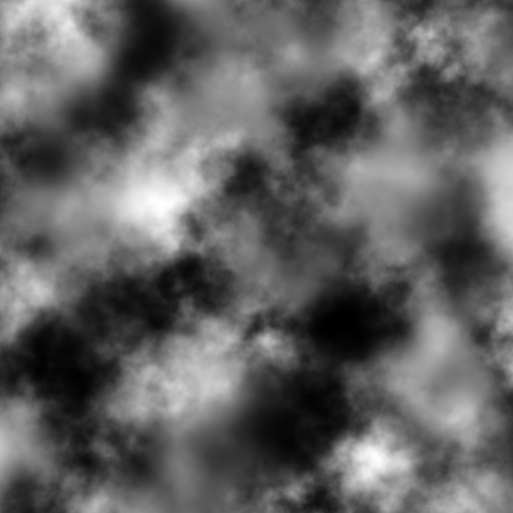
\includegraphics[width=4cm]{Ogre/1_Base_de_Ogre/5_Garder_les_pieds_sur_terre/images/terrain.png} %l'image est retaillée pour avoir une largeur de 10cm
\end{figure}

Comme vous le voyez c'est une simple image en noir et blanc, et pourtant cela suffit amplement !

En effet, si l'on utilise uniquement des niveaux de gris dans une image, chaque pixel peut prendre 256 valeurs, 0 correspondant au noir et à la hauteur la plus faible, 255 au blanc et à la plus forte altitude. On a donc 256 altitudes possibles pour notre terrain, ce qui est tout à fait honnête et suffit à la majorité des cas.

En réalité, chaque pixel possède trois valeurs, correspondant à la quantité de rouge, de vert et de bleu, chacune de ces valeurs allant de 0 à 255. Or pour les niveaux de gris, ces trois valeurs doivent être identiques, ce qui laisse 255 triplets de valeurs : (0, 0, 0) pour le noir, puis les niveaux de gris et enfin (255, 255, 255) pour le blanc).

Lors de la création d'un fichier heightmap, on fait en sorte que le point le plus haut de notre carte soit blanc et que le point le plus bas soit noir, afin d'utiliser toute la plage de valeurs disponibles dans la carte et éviter les dénivellations peu naturelles.

Pour charger un fichier heightmap, on passe par un objet Image qui va chercher le nom du fichier que vous voulez dans les ressources déjà chargées. J'utilise le fichier terrain.png, que vous pouvez trouver dans ''media/materials/textures''.

\begin{lstlisting}[caption={Chargement du fichier heightmap}]
Ogre::Image img;
img.load(''terrain.png'', Ogre::ResourceGroupManager::DEFAULT_RESOURCE_GROUP_NAME);
\end{lstlisting}






\subsubsection{Les paramètres géométriques}


Pour fournir toutes les informations dont le terrain a besoin pour être généré, on utilise sa méthode prepare()\index{prepare()}\index{Terrain!prepare()} qui prend en paramètre un Terrain::ImportData\index{ImportData}\index{Terrain!ImportData}, qui est en gros une classe contenant l'ensemble des paramètres à fournir au terrain. On va donc commencer par créer cet objet :

\begin{lstlisting}[caption={Création de l'objet ImportData pour la définition des paramètres à fournir au terrain}]
Ogre::Terrain::ImportData imp;
imp.inputImage = &img;  //recuperation de l'image
imp.terrainSize = img.getWidth();  //recuperation de la taille de l'image
imp.worldSize = 8000;  //indique la taille du terrain
imp.inputScale = 600;  //echelle adoptee pour l'altitude du terrain
imp.minBatchSize = 33; //taille min du batch pour le terrain
imp.maxBatchSize = 65; //taille max du batch pour le terrain
\end{lstlisting}

On commence par récupérer l'image et sa taille avec les lignes 2 et 3. \textbf{étant donné que les terrains sont carrés, votre image doit elle aussi être carrée}, faites attention à cela.

Ensuite, le paramètre worldSize\index{worldSize}\index{Terrain!worldSize} indique la taille du terrain, c'est-à-dire la longueur de ses côtés en unités de la scène. Plus ce nombre est grand, plus l'image est agrandie.

inputScale\index{inputScale}\index{Terrain!inputScale} correspond à l'échelle adoptée pour l'altitude du terrain. C'est la hauteur qui sépare un point de la carte représenté par un pixel noir d'un point représenté par un pixel blanc. Il doit donc être choisi en parallèle avec la taille du monde, puisque s'il est trop élevé et que le monde est trop petit, vous aurez un relief très escarpé.

Les deux dernières valeurs minBatchSize \index{minBatchSize}\index{Terrain!minBatchSize} et maxBatchSize \index{maxBatchSize}\index{Terrain!maxBatchSize} renseignent les tailles minimale et maximale de batch pour notre terrain.



\subsubsection{La Batch Size\index{Batch Size}\index{Terrain!Batch}}


Le mot anglais batch signifie ''lot'' ou ''paquet''. L'affichage de modèle 3D à l'écran consommant beaucoup de ressources, plutôt que de chercher à calculer dans les moindres détails la fa\c{c}on dont appara\^it la pelouse à l'autre bout du paysage, pour ensuite ne l'afficher que sur une toute petite surface de l'écran, le moteur va simplifier les choses et calculer de fa\c{c}on grossière l'affichage de ces objets.

Ainsi, les textures peuvent être simplifiées, mais aussi les meshs, dont l'ordinateur va réduire le nombre de vertices pour avoir moins de calculs à faire, vu que vous ne voyez pas les détails (on parle aussi de niveau de détail\index{niveau de détail}, ou LOD\index{LOD}).

Pour un terrain, le maillage pourrait donc avoir un aspect similaire à celui-ci (image issue du wiki d'Ogre3D.org) :
Image utilisateur

Le terrain est divisé en lots dont la taille varie en fonction de la distance de la caméra à ces lots. Plus on s'éloigne, plus le lot est simplifié par suppression de vertices. Lorsque plusieurs lots atteignent une taille minimale, ils sont regroupés en un seul lot, qui est à son tour simplifié progressivement si la caméra continue de reculer.

La zone o\`u se situe la caméra est la plus détaillée, le reste est simplifié.

Si la taille minimum de batch est faible, les lots adjacents auront plus facilement un niveau de détail équivalent, mais il y aura plus de lots à gérer par l'ordinateur. En revanche, si elle est élevée, on regroupe plus rapidement les lots, mais les frontières entre ceux-ci sont plus facilement visibles, car le niveau de détail peut varier plus fortement.

Les valeurs que j'ai mises sont des valeurs courantes, sachez juste que la taille maximum est de 65 et qu'\textbf{elles doivent obéir à la formule suivante :
taille=2n+1}



\subsubsection{Mise en place des textures\index{texture}\index{Terrain!texture}}

Pour gérer les textures, l'outil Terrain d'Ogre utilise des calques\index{calque}\index{Terrain!calque}. Chacun de ces calques correspond à une texture, que vous pourrez ensuite appliquer o\`u bon vous semblera.

Comme on parle de calques, autant vous dire tout de suite qu'il est possible de les superposer, de donner plus ou moins d'intensité à un calque, pour créer des effets élaborés.

Nous allons commencer avec une seule texture pour faire simple et assimiler le principe. Tout se fait à l'aide de notre importateur de données :

\begin{lstlisting}[caption={Mise en place d'une texture pour le terrain}]
//donne la taille de la liste de calques
imp.layerList.resize(1);

//donne la taille de la texture dans le monde
imp.layerList[0].worldSize = 100;  

//les deux lignes suivantes inserent chacune une texture dans notre calque
imp.layerList[0].textureNames.push\_back(''grass\_green-01\_diffusespecular.dds'');
imp.layerList[0].textureNames.push\_back(''grass\_green-01\_normalheight.dds'');
\end{lstlisting}

Ici les fonctions sont relativement explicites.

La première ligne donne la taille de la liste de calques, ici je n'en ai mis qu'un seul. La seconde ligne donne la taille de la texture dans le monde. \textbf{Plus le nombre\footnote{ce nombre est-il le nombre affecté à la taille de la texture?} est important, plus la texture sera zoomée, et inversement.}

Les deux lignes suivantes insèrent chacune une texture dans notre calque (textureNames est un vector).

Deux textures ? Je croyais qu'on mettait les textures sur des calques différents ?

En fait, on devrait plutôt dire qu'un calque contient un matériau\index{matériau}.

Les matériaux sont faits avec deux textures :

\begin{itemize}
\item une texture diffuse, qui contient les couleurs, les motifs du matériau ;
\item une texture normale, contenant des informations sur le relief du matériau.
\end{itemize}
   

La combinaison de ces deux textures permet d'avoir un matériau complet.



\subsubsection{Filtrage anisotrope\index{Filtrage anisotrope}\index{Terrain!Filtrage anisotrope}}


Je vais revenir rapidement sur le niveau de détail\index{niveau de détail}\index{Terrain!niveau de détail}, qui est réglable pour les matériaux via le filtrage de texture.

Vous pouvez régler la netteté du placage de textures sur vos meshs via un niveau de filtrage\index{niveau de filtrage}\index{Terrain!niveau de filtrage}.

On peut distinguer quatre options de filtrages, de la plus grossière à la plus précise :

\begin{itemize}
\item aucun filtrage ;
\item bilinéaire\index{niveau de filtrage!bilinéaire} ;
\item trilinéaire\index{niveau de filtrage!trilinéaire} ;
\item anisotrope\index{niveau de filtrage!anisotrope}.
\end{itemize}


Voici la différence entre un filtrage anisotrope (à gauche) et une texture sans filtrage (à droite). La différence est relativement subtile ici mais visible tout de même.

Image utilisateur

Je vous propose donc d'opter pour un filtrage anisotrope, avec une valeur de 8 (la valeur par défaut est 1 et équivaut à l'absence de filtrage). Vous devez donc rajouter ces deux lignes dans votre code, au début de la méthode createScene() par exemple.

\begin{lstlisting}[caption={Choix d'un filtrage anisotrope}]
Ogre::MaterialManager::getSingleton().setDefaultTextureFiltering(Ogre::TFO\_ANISOTROPIC);
Ogre::MaterialManager::getSingleton().setDefaultAnisotropy(8);
\end{lstlisting}

Le filtrage de textures n'est pas propre uniquement aux terrains, mais affecte toutes les textures affichées par le moteur.


\subsubsection{Chargement et nettoyage}


Une fois que les paramètres ont été définis dans l'ImportData, il ne reste qu'à préparer et charger le terrain :

\begin{lstlisting}[caption={Préparation et chargement du terrain}]
mTerrain->prepare(imp);
mTerrain->load();
\end{lstlisting}

Pour terminer et faire un peu de place en mémoire, il est conseillé d'appeler la méthode suivante qui se chargera de libérer la mémoire allouée temporairement pour la création de votre terrain. Placez donc cette ligne à la fin de la méthode createTerrain().

\begin{lstlisting}[caption={Libération de place en mémoire}]
mTerrain->freeTemporaryResources();
\end{lstlisting}

Compilez et lancez l'application pour obtenir un joli paysage !
































%---------------------------------------------------------------------------------------------------------------


\section{Le plaquage de textures}


Ogre nous permet d'utiliser différents calques pour nos matériaux. On va pouvoir mettre les calques les uns sur les autres, modifier leur opacité pour avoir une texture plus ou moins visible, tout en décidant de la zone o\`u l'on veut appliquer la texture.

La première étape consiste à rajouter des calques dans notre liste, avant de créer le terrain. Remplacez le bloc que vous aviez par le code suivant, afin d'ajouter deux nouveaux matériaux.



\begin{lstlisting}[caption={Ajout de calques}]
imp.layerList.resize(3);

imp.layerList[0].worldSize = 100;
imp.layerList[0].textureNames.push_back("grass_green-01_diffusespecular.dds");
imp.layerList[0].textureNames.push_back("grass_green-01_normalheight.dds");

imp.layerList[1].worldSize = 30;
imp.layerList[1].textureNames.push_back("growth_weirdfungus-03_diffusespecular.dds");
imp.layerList[1].textureNames.push_back("growth_weirdfungus-03_normalheight.dds");

imp.layerList[2].worldSize = 200;
imp.layerList[2].textureNames.push_back("dirt_grayrocky_diffusespecular.dds");
imp.layerList[2].textureNames.push_back("dirt_grayrocky_normalheight.dds");

mTerrain->prepare(imp);
mTerrain->load();
\end{lstlisting}

Par défaut, c'est uniquement le premier matériau qui est affiché donc si vous exécutez le code maintenant, rien n'aura changé sur votre terrain.  Il est donc nécessaire d'ajouter quelques lignes pour dire de quelle fa\c{c}on nous voulons faire notre plaquage de texture.\newline

Le principe est simple à comprendre, chaque calque d'un terrain possède un objet TerrainLayerBlendMap\index{TerrainLayerBlendMap}\index{Terrain!TerrainLayerBlendMap} (que j'appellerai dorénavant Blend Map\index{Blend Map}) qui exprime la fa\c{c}on dont le calque est fusionné avec les calques inférieurs (le calque le plus bas est le calque 0).

Cette fusion\index{fusion de calques}\index{Terrain!fusion de calques} est simplement une affaire de transparence. Les calques sont placés les uns sur les autres, et la composante transparente indique si la texture en dessous est plus ou moins visible. Il est de plus possible de faire varier la transparence du calque en chaque point de celui-ci, ce qui permet d'avoir un placage par zone.\newline

à la suite du bloc de code précédent, commencez par récupérer les Blend Map correspondant au calque numéro 1, que nous venons d'ajouter (nous nous occuperons du second ensuite).

\begin{lstlisting}[caption={Récupération du Blend Map pour le premier terrain}]
Ogre::TerrainLayerBlendMap* blendMap1 = mTerrain->getLayerBlendMap(1);
\end{lstlisting}

Nous allons commencer par plaquer une seule texture au-dessus de l'herbe, sur toute la surface de notre terrain.

L'idée est de parcourir l'ensemble des points du calque avec deux boucles for (il y a autant de points qu'il y avait de pixels dans notre heightmap) et de leur attribuer la transparence désirée, entre 1 (totalement opaque) et 255 (transparent).

La valeur la plus faible est bien 1 et non 0. Si vous mettez 0, la texture est transparente !

\begin{lstlisting}[caption={Attribution de la transparence désirée sur tous les points du calque}]
float* pBlend1 = blendMap1->getBlendPointer();

for (Ogre::uint16 y = 0; y < mTerrain->getLayerBlendMapSize(); ++y)
{
    for (Ogre::uint16 x = 0; x < mTerrain->getLayerBlendMapSize(); ++x)
    {   
        // opacite desiree pour le point courant
        *pBlend1++ = 150;
    }
}
\end{lstlisting}















Pour terminer, il faut mettre à jour notre Blend Map en appelant les méthodes dirty()\index{dirty()}\index{Blend Map!dirty()} puis update()\index{update()}\index{Blend Map!update()}. La première sert à préciser que les données de la Blend map sont obsolètes et doivent être mises à jour, tandis que la seconde fait effectivement la mise à jour.

Si vous n'appelez pas d'abord dirty(), update() n'aura aucun effet.

\begin{lstlisting}[caption={Mise à jour de la Blend Map}]
blendMap1->dirty();
blendMap1->update();
\end{lstlisting}

Je vous mets le code complet de la méthode createTerrain() si vous voulez vérifier que tout est en ordre :

\begin{lstlisting}[caption={createTerrain (code complet)}]
mTerrain = OGRE_NEW Ogre::Terrain(mSceneMgr);

// options globales
mGlobals = OGRE_NEW Ogre::TerrainGlobalOptions();
mGlobals->setMaxPixelError(10);
mGlobals->setCompositeMapDistance(8000);
mGlobals->setLightMapDirection(mLight->getDerivedDirection());
Globals->setCompositeMapAmbient(mSceneMgr->getAmbientLight());
mGlobals->setCompositeMapDiffuse(mLight->getDiffuseColour());
Ogre::Image img;
img.load("terrain.png", Ogre::ResourceGroupManager::DEFAULT_RESOURCE_GROUP_NAME);

// informations geometriques
Ogre::Terrain::ImportData imp;
imp.inputImage = &img;
imp.terrainSize = img.getWidth();
imp.worldSize = 8000;
imp.inputScale = 600;
imp.minBatchSize = 33;
imp.maxBatchSize = 65;

// textures
imp.layerList.resize(3);
imp.layerList[0].worldSize = 100;
imp.layerList[0].textureNames.push_back("grass_green-01_diffusespecular.dds");
imp.layerList[0].textureNames.push_back("grass_green-01_normalheight.dds");
imp.layerList[1].worldSize = 30;
imp.layerList[1].textureNames.push_back("growth_weirdfungus-03_diffusespecular.dds");
imp.layerList[1].textureNames.push_back("growth_weirdfungus-03_normalheight.dds");
imp.layerList[2].worldSize = 200;
imp.layerList[2].textureNames.push_back("dirt_grayrocky_diffusespecular.dds");
imp.layerList[2].textureNames.push_back("dirt_grayrocky_normalheight.dds");
mTerrain->prepare(imp);35mTerrain->load();

// plaquage de texture
Ogre::TerrainLayerBlendMap* blendMap1 = mTerrain->getLayerBlendMap(1);
float* pBlend1 = blendMap1->getBlendPointer();
for (Ogre::uint16 y = 0; y < mTerrain->getLayerBlendMapSize(); ++y)
{
    for (Ogre::uint16 x = 0; x < mTerrain->getLayerBlendMapSize(); ++x)
    {
        *pBlend1++ = 150;
    }
}

blendMap1->dirty();
blendMap1->update();

mTerrain->freeTemporaryResources();
\end{lstlisting}

Vous pouvez maintenant exécuter l'application ! Profitez-en pour vérifier en vous approchant du sol que l'on distingue bien l'herbe et par-dessus la terre.
Image utilisateur

On va tout de suite essayer de faire quelque chose de plus esthétique.

Pour cela, maintenant que vous avez saisi les grandes étapes, je vous propose un mini-TP pour vous entra\^iner.








\subsection{Au boulot !}



\subsubsection{Objectif}

Une image vaut s\^urement mieux qu'un long discours, voici donc ce que vous allez devoir obtenir :
Image utilisateur

L'idée est de texturer le terrain en fonction de l'altitude. Si l'on est en dessous d'un certain seuil, il n'y a que de la terre qui appara\^it ; au-dessus, on a de l'herbe.



\subsubsection{Indications}

Je vous donne tout de même les méthodes qui sont utiles, notamment pour trouver l'altitude du terrain en fonction de la position :

\begin{lstlisting}[caption={méthode getHeightAtTerrainPosition pour trouver l'altitude du terrain en fonction de la position }]
float Ogre::Terrain::getHeightAtTerrainPosition(Ogre::Real x, Ogre::Real y)
\end{lstlisting}

Cette fonction retourne l'altitude en fonction de la position, sachant que x et y sont compris entre 0 et 1.

Pour récupérer ces deux valeurs, on utilise une méthode de TerrainLayerBlendMap qui convertit les coordonnées de l'image en coordonnées du terrain (celles dont vous avez besoin) :

\begin{lstlisting}[caption={Méthode convertImageToTerrainSpace pour convertir les coordonnées de l'image en coordonnées du terrain}]
void Ogre::TerrainLayerBlendMap::convertImageToTerrainSpace(size_t x, size_t y, Ogre::Real * outX, Ogre::Real * outY)
\end{lstlisting}


Enfin, je vous laisse choisir l'altitude limite entre l'herbe et la terre. Vous avez toutes les cartes en mains maintenant.

























\subsubsection{Correction}

Comme avez d\^u le deviner, tout se passe dans les deux boucles for.

Pour chaque point parcouru, on recherche ses coordonnées dans le repère du terrain, puis on récupère la hauteur, que l'on compare à notre hauteur limite. Si on est en dessous, on affiche la texture de terre avec une opacité maximum, sinon on ne fait qu'incrémenter le pointeur de la Blend map.

Voici donc le code modifié :

\begin{lstlisting}[caption={Attribution de la transparence désirée sur tous les points du calque selon leur position}]
for (Ogre::uint16 y = 0; y < mTerrain->getLayerBlendMapSize(); ++y)
{
    for (Ogre::uint16 x = 0; x < mTerrain->getLayerBlendMapSize(); ++x)
    {
        Ogre::Real terrainX, terrainY;
        blendMap1->convertImageToTerrainSpace(x, y, &terrainX, &terrainY);
        Ogre::Real height = mTerrain->getHeightAtTerrainPosition(terrainX, terrainY);
        if(height < 200)
            *pBlend1 = 1;
        pBlend1++;
    }
}
\end{lstlisting}

Vous pouvez aussi bien s\^ur récupérer la Blend map numéro 2 plus haut pour voir le résultat avec une autre texture, c'est ce que j'ai fait pour obtenir l'image référence pour le TP.








\subsubsection{Code}

Ci-dessous le trouve le code de la metohde createTerrain et le resultat obtenu:

\begin{lstlisting}[caption={createTerrain}]
void PremiereApplication::createTerrain()
{    
    Ogre::Vector3 lightdir(0.55f, -0.3f, 0.75f);
    
    mLight = mSceneMgr->createLight("terrainLight");
    mLight->setType(Light::LT_DIRECTIONAL);
    mLight->setDirection(lightdir);
    mLight->setDiffuseColour(Ogre::ColourValue::White);
    mLight->setSpecularColour(Ogre::ColourValue(0.4f, 0.4f, 0.4f)); 
    
    mGlobals = OGRE_NEW Ogre::TerrainGlobalOptions();
    mGlobals->setMaxPixelError(8); /**<specifie la precision de rendu (en nbr de pixel) du terrain*/    
    
    //application des reglages de lumiere aux options globales
    mGlobals->setLightMapDirection(mLight->getDerivedDirection());
    mGlobals->setCompositeMapDistance(3000);
    mGlobals->setCompositeMapAmbient(mSceneMgr->getAmbientLight());
    mGlobals->setCompositeMapDiffuse(mLight->getDiffuseColour());    
    
    mTerrain = OGRE_NEW Ogre::Terrain(mSceneMgr);/**<Creation du terrain*/
    
    Ogre::Image img;
    img.load("terrain.png", Ogre::ResourceGroupManager::DEFAULT_RESOURCE_GROUP_NAME);/**<Chargement de l'image Heighmaps contenant les infos pour le relief*/
    
    ///Mise en place des proprietes generales du terrain
    Ogre::Terrain::ImportData imp;/**<creation de l'objet qui contiendra toutes les infos pour le terrain*/
    imp.inputImage = &img;/**<recuperation de l image*/
    imp.terrainSize = img.getWidth();/**<recuperation de la taille de l image (les terrains sont carres, l'image doit donc etre carree)*/

    imp.worldSize = 8000;/**<taille du terrain en unites de la scene (plus ce nbre est grande, plus l'image est grande)*/
    imp.inputScale = 600;/**<echelle adoptee pour l altitude du terrain (difference entre un pt a l'altitude 0 (pt en blanc ds terrain.png) et un point a l'altitude max (pt en noir))*/
    imp.minBatchSize = 33;/**<taille min du batch pour le terrain*/
    imp.maxBatchSize = 65;/**<taille max du batch pour le terrain*/
    
    ///Mise en place des textures
    imp.layerList.resize(1);/**<donne la taille de la liste des calques*/
    imp.layerList[0].worldSize = 100;/**<donne la taille de la texture ds le monde (plus le nbre est gd plus la texture est zoomee)*/
    ///insertion de textures dans notre calque
    imp.layerList[0].textureNames.push_back("grass_green-01_diffusespecular.dds");/**>contient les couleurs, les motifs du materiau*/
    imp.layerList[0].textureNames.push_back("grass_green-01_normalheight.dds");/**<contient des infos sur le relief du materiau*/
    
    ///Filtrage anisotropique (affecte toutes les textures)
    Ogre::MaterialManager::getSingleton().setDefaultTextureFiltering(Ogre::TFO_ANISOTROPIC);
    Ogre::MaterialManager::getSingleton().setDefaultAnisotropy(8);
    
    ///Rajout de calques dans notre liste
    imp.layerList.resize(3);
    imp.layerList[0].worldSize = 100;
    imp.layerList[0].textureNames.push_back("grass_green-01_diffusespecular.dds");
    imp.layerList[0].textureNames.push_back("grass_green-01_normalheight.dds");
    imp.layerList[1].worldSize = 30;
    imp.layerList[1].textureNames.push_back("growth_weirdfungus-03_diffusespecular.dds");
    imp.layerList[1].textureNames.push_back("growth_weirdfungus-03_normalheight.dds");
    imp.layerList[2].worldSize = 200;
    imp.layerList[2].textureNames.push_back("dirt_grayrocky_diffusespecular.dds");
    imp.layerList[2].textureNames.push_back("dirt_grayrocky_normalheight.dds");
    
    mTerrain->prepare(imp);/**<on fournit toutes les informations necessaires au terrain*/
    mTerrain->load();/**<chragement du terrain*/    
    
    ///recuperation du blend map pour le premier terrain
    Ogre::TerrainLayerBlendMap* blendMap2 = mTerrain->getLayerBlendMap(2);/**<recuperation du blend map*/
    
    ///plaquage de la texture..
    float* pBlend2 = blendMap2->getBlendPointer();
    ///..en fonction de l'altitude
    for (Ogre::uint16 y = 0; y < mTerrain->getLayerBlendMapSize(); ++y)
    {
        for (Ogre::uint16 x = 0; x < mTerrain->getLayerBlendMapSize(); ++x)
        {
            Ogre::Real terrainX, terrainY;
            
            blendMap2->convertImageToTerrainSpace(x, y, &terrainX, &terrainY);
            Ogre::Real height = mTerrain->getHeightAtTerrainPosition(terrainX, terrainY);
            
            //en general l'herbe se trouve en basse altitude
            if(height > 200)
                *pBlend2 = 1;
            
            pBlend2++;
        }
    }
    
    blendMap2->dirty();/**<precise que les donnees de la blend Map st obsoletes*/
    blendMap2->update();/**<fait la mise a jour des donnees de la blend map*/ 
    
    mTerrain->freeTemporaryResources();/**<liberation de la memoire allouee temporairement*/
}

\end{lstlisting}




\begin{lstlisting}[caption={PremiereApplication.h}]

using namespace std;

#include <ExampleApplication.h>
#include <OgreMovableObject.h>
#include "InputListener.h"

#include <Terrain/OgreTerrain.h>

class PremiereApplication : public ExampleApplication
{    
    public:
        Terrain *mTerrain;                      /**<gerera les proprietes de notre terrain*/
        Ogre::TerrainGlobalOptions *mGlobals;   /**<objet obligatoire pr la gestion des terrains, definira les proprietes generales pour le terrain (ex: eclairage)*/
        Light *mLight;                          /**<contiendra les prorietes de la lumiere*/
        
        /** Cree la scene avec une tete d'Ogre flottant sur un carre de pelouse
         */
        void createScene();
        
        /** Cree et place la camera
         */
        void createCamera();
        
        /** Cree une seconde vue de la scene
         */
        void createViewports();

        /** Gere les entrees 
         */
        void createFrameListener();
        
        /** Cree une lumiere selon le parametre
         @param luxType - type de lumiere desiree 
         @param lux - instance de lumiere 
         @return distance to point
         */
        //void createLux(std::string luxType, MovableObject *lux);
        
        /** Initialise le terrain
         */
        void createTerrain();
};
\end{lstlisting}













\begin{lstlisting}[caption={CMakeLists.txt}]
project(helloworld)
cmake_minimum_required(VERSION 2.6)

set(CMAKE_MODULE_PATH "/usr/share/OGRE/cmake/modules")

set(CMAKE_CXX_FLAGS "-Wall -std=c++11 -g")

# Il s'agit du tutoriel d'exemple, qui utilise quelques fichiers prdfini de Ogre. Il faut indiquer a cmake ou se trouvent les includes en question
include_directories ("include")

# Bien sur, pour compiler Ogre, il faut le chercher, et dfinir le rpertoire contenant les includes.
find_package(OGRE REQUIRED)
include_directories (${OGRE_INCLUDE_DIRS})

if (OGRE_Overlay_FOUND)
# append OgreOverlay to the end of the OGRE_LIBRARIES variable
  set(OGRE_LIBRARIES ${OGRE_LIBRARIES} ${OGRE_Overlay_LIBRARIES})
  message(STATUS "Found OGRE_Terrain: ${OGRE_Overlay_LIBRARIES}")
else (OGRE_Overlay_FOUND)
  message(SEND_ERROR "OgreOverlay Library not found.")
endif(OGRE_Overlay_FOUND)

#Inclusion de la lib libOgreTerrain.so
if (OGRE_Terrain_FOUND)
  set(OGRE_LIBRARIES ${OGRE_LIBRARIES} ${OGRE_Terrain_LIBRARIES})
  message(STATUS "Found OGRE_Terrain: ${OGRE_Terrain_LIBRARIES}")
else (OGRE_Terrain_FOUND)
  message(SEND_ERROR "OgreTerrain Library not found.")
endif(OGRE_Terrain_FOUND)


#Inclusion de la lib libOgrePaging.so
if (OGRE_Paging_FOUND)
  set(OGRE_LIBRARIES ${OGRE_LIBRARIES} ${OGRE_Paging_LIBRARIES})
  message(STATUS "Found OGRE_Paging: ${OGRE_Paging_LIBRARIES}")
else (OGRE_Paging_FOUND)
  message(SEND_ERROR "OgrePaging Library not found.")
endif(OGRE_Paging_FOUND)


# L'exemple depend aussi de OIS, une lib pour gerer la souris, clavier, joystick...
find_package(OIS REQUIRED)

# On dfinit les sources qu'on veut compiler
SET( SOURCES
  src/InputListener.cpp  
  src/PremiereApplication.cpp
  src/main.cpp
)

# On les compile
add_executable (
  premiereapp ${SOURCES}
)

message(STATUS "OGRE Libraries used to link are ${OGRE_LIBRARIES}")

# Et pour finir, on lie l'executable avec les librairies que find_package nous a gentillement trouve.
target_link_libraries(premiereapp ${OGRE_LIBRARIES} ${OIS_LIBRARY} -lboost_system)



set( RESOURCES_FILE
  media/
  resources/ogre.cfg
  resources/plugins.cfg
  resources/resources.cfg
)

# do the copying
foreach( file_i ${RESOURCES_FILE})
    add_custom_command(
      TARGET premiereapp
      POST_BUILD
      COMMAND cp -R ${CMAKE_SOURCE_DIR}/${file_i} ${CMAKE_BINARY_DIR}
      COMMENT "copy file ${file_i}"
      )
endforeach( file_i )

\end{lstlisting}





Et on obtiend:
\begin{figure}[hbtp]
\caption{Terrain.png}
\centering
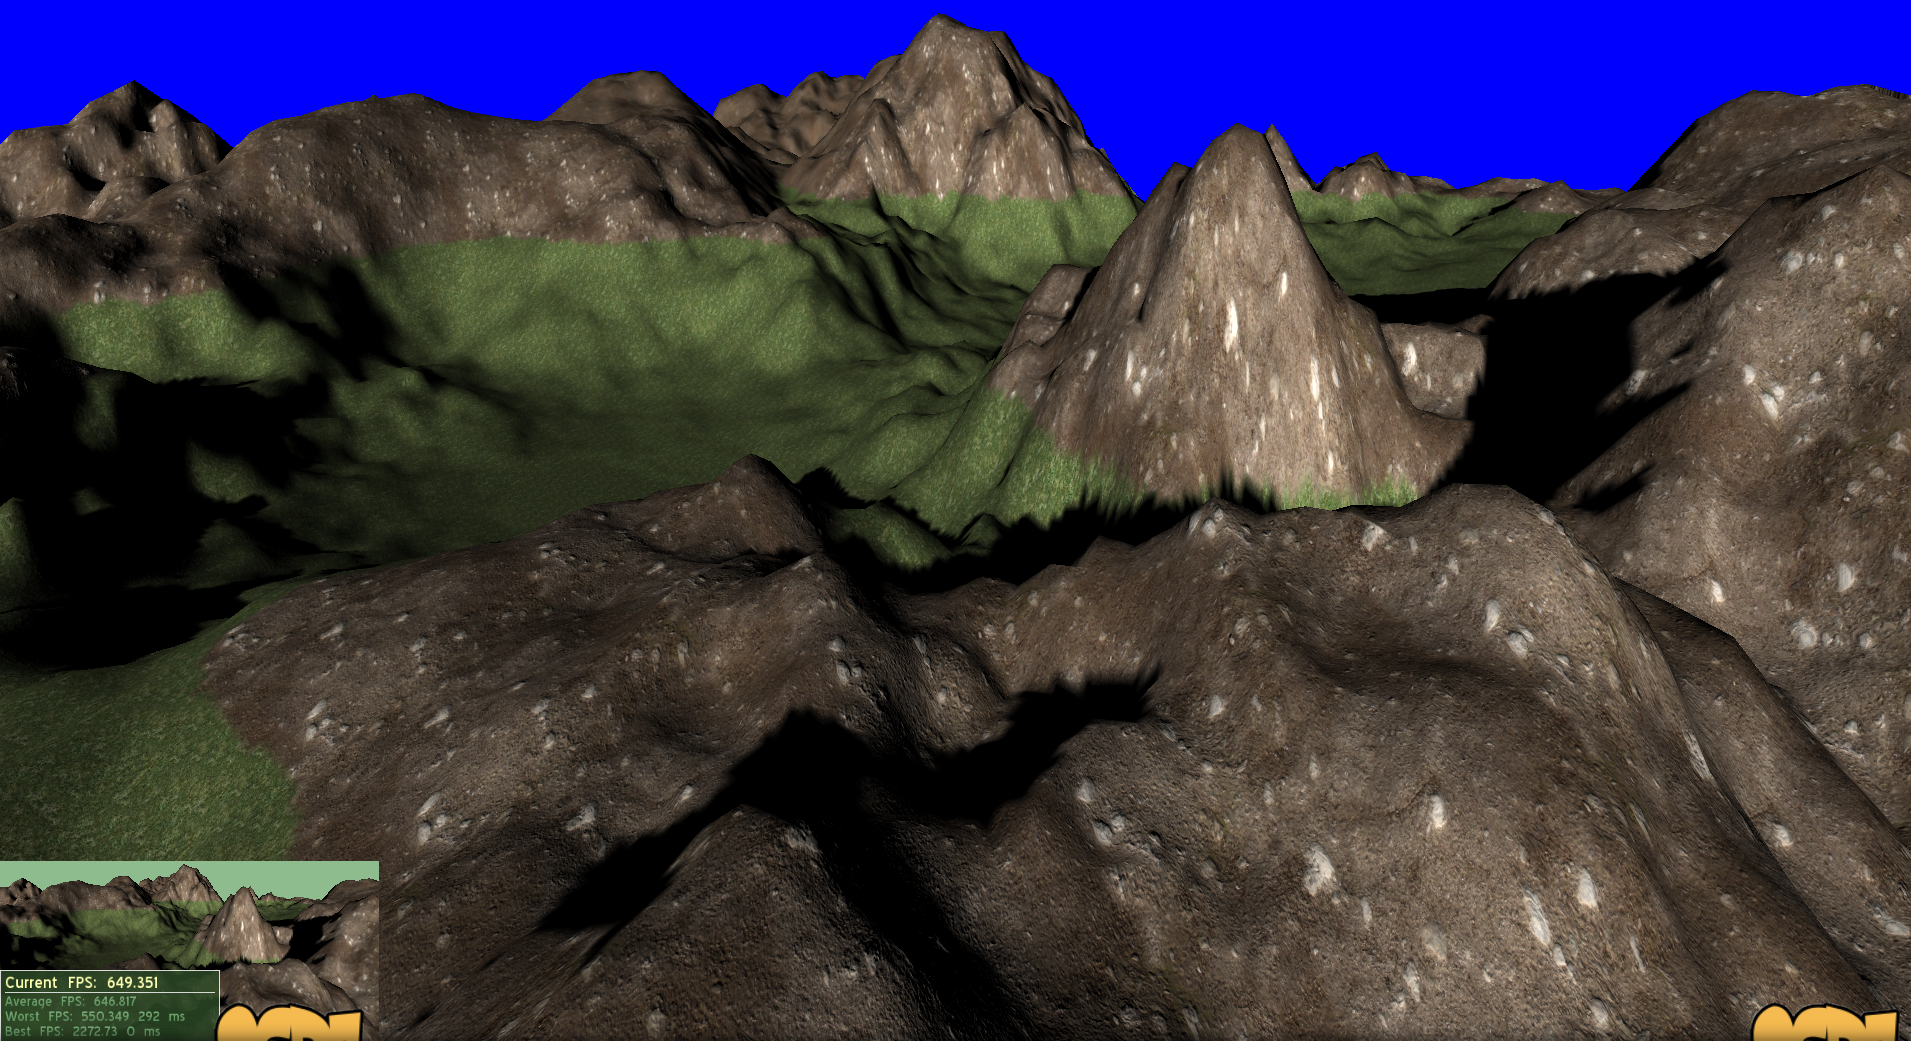
\includegraphics[width=8cm]{Ogre/1_Base_de_Ogre/5_Garder_les_pieds_sur_terre/images/Differentes_textures_selon_altitude1.png} %l'image est retaillée pour avoir une largeur de 10cm
\end{figure}




















\subsection{Pour aller plus loin}


Sur le même principe, nous allons voir comment appliquer deux textures différentes sur une petite largeur, à une altitude donnée.

Ceci peut être utile si vous voulez réaliser des étendues d'eau dans votre terrain : au bord de l'eau, il y a de la boue, un peu au-dessus, de la terre sèche, puis ensuite l'herbe reprend ses droits. C'est ce que nous allons faire, avec une opacité progressive, mais sans l'eau, ce sera pour plus tard.

Nous devons commencer par récupérer un pointeur sur notre seconde Blend Map pour pouvoir gérer la seconde texture en plus de la première. Il y a donc deux lignes à rajouter en conséquence avant les boucles.




\begin{lstlisting}[caption={Récupération des Blend Map pour le premier et le second terrain}]
Ogre::TerrainLayerBlendMap* blendMap1 = mTerrain->getLayerBlendMap(1);
Ogre::TerrainLayerBlendMap* blendMap2 = mTerrain->getLayerBlendMap(2);

float* pBlend1 = blendMap1->getBlendPointer();
float* pBlend2 = blendMap2->getBlendPointer();
\end{lstlisting}

Définissons aussi deux variables pour chacune des textures : la hauteur à laquelle se situe la texture et la largeur de la bande que l'on veut obtenir.

\begin{lstlisting}[caption={}]
Ogre::Real minHeight1 = 70;
Ogre::Real fadeDist1 = 40;
Ogre::Real minHeight2 = 70;
Ogre::Real fadeDist2 = 15;
\end{lstlisting}

Dans la boucle, on déclare trois variables : deux coordonnées du terrain et la transparence pour le point actuel.

\begin{lstlisting}[caption={}]
Ogre::Real terrainX, terrainY, transparence;
\end{lstlisting}

On récupère ensuite la hauteur du terrain comme précédemment.

\begin{lstlisting}[caption={}]
blendMap1->convertImageToTerrainSpace(x, y, &terrainX, &terrainY);
Ogre::Real height = mTerrain->getHeightAtTerrainPosition(terrainX, terrainY);
\end{lstlisting}

Ensuite, pour chaque texture, on calcule la différence entre la hauteur du point actuel et la hauteur que l'on veut pour la texture, divisée par la largeur de la bande. Si le point est censé être recouvert par la texture, ce nombre sera donc compris entre 0 et 1.

On utilise ensuite la méthode statique Clamp() qui a pour prototype :

\begin{lstlisting}[caption={Utilisation de la méthode statique Clamp()}]
static T Ogre::Math::Clamp(T val, T minval, T maxval)
\end{lstlisting}

Si val est inférieure à minval, la fonction retourne minval ; si val est supérieure à maxval, on retourne maxval. Si val est dans l'intervalle, on la retourne directement.

Comme on ne veut afficher que les points dont la valeur calculée précédemment est comprise entre 0 et 1, on va utiliser cette méthode pour ''couper'' toutes les valeurs en dehors de l'intervalle.

\begin{lstlisting}[caption={}]
transparence = (height - minHeight1) / fadeDist1;
transparence = Ogre::Math::Clamp(transparence, (Ogre::Real)0, (Ogre::Real)1);
\end{lstlisting}

Pour terminer, on multiplie transparence par 255 pour avoir une valeur comprise entre 0 et 255.

\begin{lstlisting}[caption={}]
*pBlend1++ = transparence * 255;
\end{lstlisting}

On observe que si transparence est à l'extérieur de l'intervalle [0 ; 1] après le premier calcul, Clamp retournera 0 ou 1. Quand on multiplie par 255, on obtient donc 0 ou 255, qui sont les deux valeurs pour lesquelles la texture est transparente. Mission accomplie !

On copie ces trois lignes pour la seconde texture, et on obtient le code suivant dans nos boucles :

\begin{lstlisting}[caption={}]
for (Ogre::uint16 y = 0; y < mTerrain->getLayerBlendMapSize(); ++y)
{
    for (Ogre::uint16 x = 0; x < mTerrain->getLayerBlendMapSize(); ++x)
    {
        Ogre::Real terrainX, terrainY, transparence;
        blendMap1->convertImageToTerrainSpace(x, y, &terrainX, &terrainY);
        Ogre::Real height = mTerrain->getHeightAtTerrainPosition(terrainX, terrainY);
        transparence = (height - minHeight1) / fadeDist1;
        transparence = Ogre::Math::Clamp(transparence, (Ogre::Real)0, (Ogre::Real)1);
        *pBlend1++ = transparence * 255;
        transparence = (height - minHeight2) / fadeDist2;
        transparence = Ogre::Math::Clamp(transparence, (Ogre::Real)0, (Ogre::Real)1);
        *pBlend2++ = transparence * 255;
    }
}
\end{lstlisting}

Pensez à mettre à jour la seconde Blend Map une fois que les modifications sont terminées :

\begin{lstlisting}[caption={}]
blendMap1->dirty();
blendMap2->dirty();
blendMap1->update();
blendMap2->update();
\end{lstlisting}




\subsubsection{Code}
Les seules choses à changer sont le plaquage de texture:


\begin{lstlisting}[caption={Plaquage de textures sur zone}]
...
    ///pour definir des bandes d'altitude avec une texture differente
    Ogre::Real minHeight1 = 70;
    Ogre::Real fadeDist1 = 40;
    Ogre::Real minHeight2 = 70;
    Ogre::Real fadeDist2 = 15;
    
    
    ///recuperation du blend map pour le premier terrain
    Ogre::TerrainLayerBlendMap* blendMap1 = mTerrain->getLayerBlendMap(1);/**<recuperation du blend map*/
    Ogre::TerrainLayerBlendMap* blendMap2 = mTerrain->getLayerBlendMap(2);/**<recuperation du blend map*/
    
    ///plaquage de la texture..
    float* pBlend1 = blendMap1->getBlendPointer();
    float* pBlend2 = blendMap2->getBlendPointer();
    ///..en fonction de l'altitude
    for (Ogre::uint16 y = 0; y < mTerrain->getLayerBlendMapSize(); ++y)
    {
        for (Ogre::uint16 x = 0; x < mTerrain->getLayerBlendMapSize(); ++x)
        {
            Ogre::Real terrainX, terrainY, transparence;
            
            blendMap1->convertImageToTerrainSpace(x, y, &terrainX, &terrainY);
            Ogre::Real height = mTerrain->getHeightAtTerrainPosition(terrainX, terrainY);
            
            transparence = (height - minHeight1) / fadeDist1;
            transparence = Ogre::Math::Clamp(transparence, (Ogre::Real)0, (Ogre::Real)1);
            *pBlend1++ = transparence * 255;
            
            transparence = (height - minHeight2) / fadeDist2;
            transparence = Ogre::Math::Clamp(transparence, (Ogre::Real)0, (Ogre::Real)1);
            *pBlend2++ = transparence * 255;
        }
    }
    
    blendMap1->dirty();/**<precise que les donnees de la blend Map st obsoletes*/
    blendMap1->update();/**<fait la mise a jour des donnees de la blend map*/
    blendMap2->dirty();/**<precise que les donnees de la blend Map st obsoletes*/
    blendMap2->update();/**<fait la mise a jour des donnees de la blend map*/ 
...
\end{lstlisting}



Et on obtiend:
\begin{figure}[hbtp]
\caption{Terrain.png}
\centering
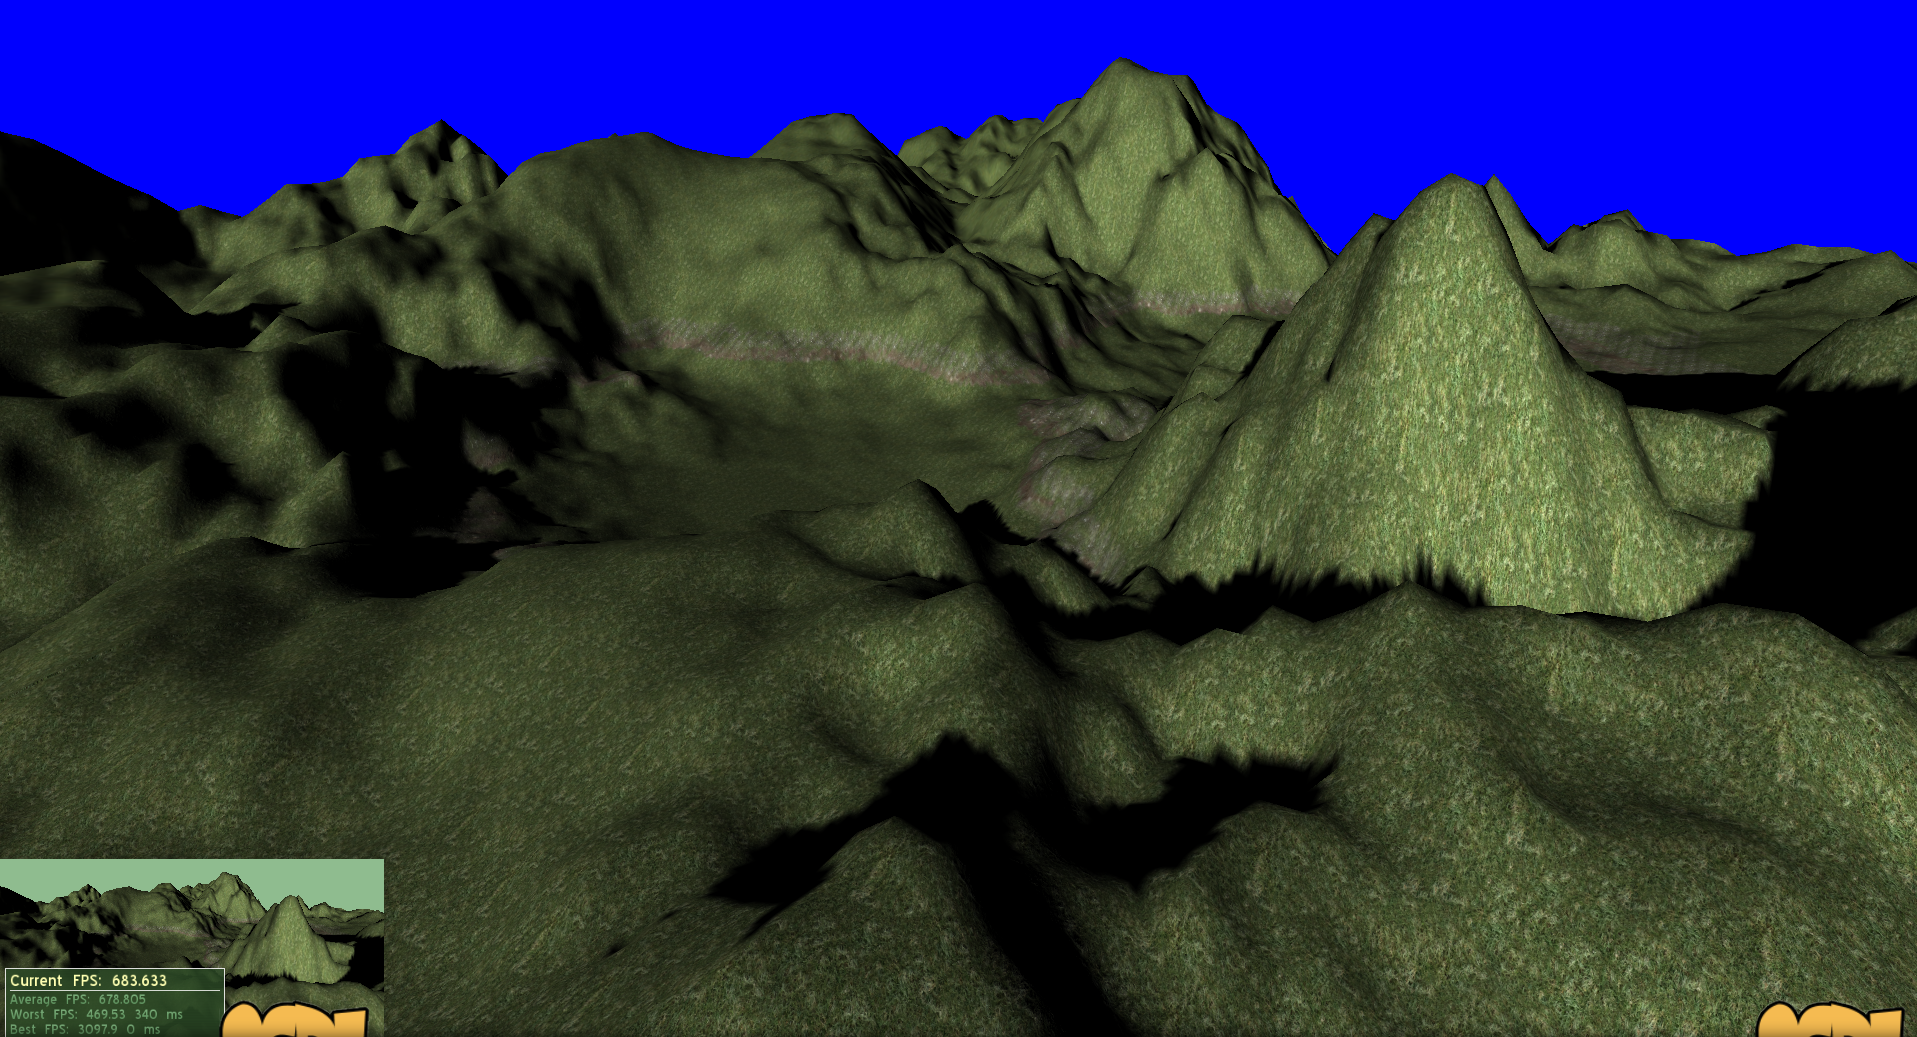
\includegraphics[width=8cm]{Ogre/1_Base_de_Ogre/5_Garder_les_pieds_sur_terre/images/Differentes_textures_selon_altitude2.png} %l'image est retaillée pour avoir une largeur de 10cm
\end{figure}








%140522
%A relire, corriger et indexer à partir d ici
%---------------------------------------------------------------------------------------------------------------
\section{Les groupes de terrains}

Un groupe de terrains\index{groupe de terrains} (ou TerrainGroup\index{TerrainGroup}) range les terrains comme dans un tableau à deux dimensions. Dans le groupe, tous les terrains doivent avoir la même taille, afin de pouvoir les aligner dans une grille.



\subsection{Création}

On commence par ajouter un include au début de la classe puis on remplace notre instance de Terrain par un TerrainGroup, ensuite on l'initialisera dans notre méthode createTerrain() :

\begin{lstlisting}[caption={TerrainGroup: include et création}]
#include <Ogre/Terrain/OgreTerrainGroup.h>
//...
Ogre::TerrainGroup *mTerrainGroup;
\end{lstlisting}

Après les lignes permettant de charger l'image heightmap dans la méthode createTerrain()\index{createTerrain()}, insérez les lignes suivantes.

\begin{lstlisting}[caption={}]
mTerrainGroup = OGRE_NEW Ogre::TerrainGroup(mSceneMgr, Ogre::Terrain::ALIGN_X_Z, img.getWidth(), 8000);

//On definit ensuite la position de l'origine du groupe de terrains
mTerrainGroup->setOrigin(Ogre::Vector3::ZERO);

//nom (et l'extension) que l'on veut attribuer a nos fichiers qui seront crees pour sauvegarder les terrains
mTerrainGroup->setFilenameConvention(Ogre::String("TerrainDuZero"), Ogre::String("dat"));
\end{lstlisting}

Les paramètres à fournir au TerrainGroup sont
\begin{itemize}
\item le Scene manager,
\item l'alignement du terrain\index{ALIGN\_X\_Z}\index{Terrain!ALIGN\_X\_Z}\index{alignement du terrain} par rapport au repère global (vous pouvez créer un terrain vertical, par exemple),
\item la taille des heightmaps utilisées\index{getWidth()}\index{heightmaps!getWidth()}, 
\item la taille d'un terrain.
\end{itemize}

On définit ensuite la position de l'origine du groupe de terrains\index{setOrigin()}\index{TerrainGroup!setOrigin()}, puis le nom\index{setFilenameConvention()}\index{TerrainGroup!setFilenameConvention()} (et l'extension) que l'on veut attribuer à nos fichiers qui seront créés pour sauvegarder les terrains par la suite.

Pour les données des terrains enregistrées dans un objet ImportData, nous allons modifier un peu le fonctionnement du programme. On récupère en fait directement une référence sur un ImportData fourni par le TerrainGroup\index{getDefaultImportSettings()}\index{TerrainGroup!getDefaultImportSettings()}, que l'on modifie directement et qui sera valable pour l'ensemble des terrains du groupe. à noter que la ligne de définition de la heightmap n'est plus utile ici, cela sera indiqué lors de la création des terrains.

\begin{lstlisting}[caption={}]
Ogre::Terrain::ImportData& imp = mTerrainGroup->getDefaultImportSettings();
imp.terrainSize = img.getWidth();
imp.worldSize = 8000;
imp.inputScale = 600;
imp.minBatchSize = 33;
imp.maxBatchSize = 65;
\end{lstlisting}

Il est maintenant temps de créer les terrains du groupe. On définit la taille du groupe et pour chaque case, on appelle une méthode definirTerrain() définie plus bas qui s'occupera de créer chaque terrain indépendamment.

\begin{lstlisting}[caption={Création des terrains du groupe}]
int largeur = 2, longueur = 2;

for(int x = 0; x < largeur; x++)
{
    for(int y = 0; y < longueur; y++)
    {
        definirTerrain(x, y);
    }
}
mTerrainGroup->loadAllTerrains(true);
\end{lstlisting}

Le groupe se charge pour terminer d'appeler les méthodes load()\index{load()} de chaque terrain à travers la méthode loadAllTerrains()\index{loadAllTerrains()}. Cette méthode prend un booléen en paramètre qui indique si le chargement doit être synchrone, c'est-à-dire exécuté dans un seul thread (le thread principal ici). Par défaut cette valeur est fausse, c'est-à-dire que les terrains sont chargés dans plusieurs threads si c'est possible.

Le chargement devient vite très lourd si l'on ajoute beaucoup de terrains aux groupes. Nous verrons plus bas comment accélérer le chargement.

Maintenant, nous devons écrire la méthode definirTerrain() qui utilise la méthode defineTerrain()\index{defineTerrain()}\index{TerrainGroup!defineTerrain()} de TerrainGroup. Celle-ci va prendre 3 paramètres : les deux coordonnées du terrain dans le groupe de terrains (sa position sur la grille, donc) et l'image heightmap utilisée pour ce terrain. Les coordonnées du terrain au sein du groupe peuvent être négatives.

Juste avant d'appeler le terrain, on va faire une vérification sur les coordonnées : si l'abscisse du terrain est impaire, on inverse l'image suivant l'axe Y, si l'ordonnée est impaire, on inverse l'image cette fois-ci selon l'axe X. Cela permet aux terrains du groupe de ne pas avoir de différence d'altitude lors des jointures. Si vous utilisez des heightmaps\index{heightmaps} différents sur les terrains du groupe (ce qui sera probablement le cas), vous devrez faire attention à ce que les altitudes des bords correspondent pour éviter les trous à ces endroits.

\begin{lstlisting}[caption={PremiereApplication.definirTerrain}]
void PremiereApplication::definirTerrain(int x, int y)
{
    Ogre::Image img;
    img.load("terrain.png", Ogre::ResourceGroupManager::DEFAULT_RESOURCE_GROUP_NAME);

    if(x % 2 != 0)
        img.flipAroundY();

    if(y % 2 != 0)
        img.flipAroundX();

    mTerrainGroup->defineTerrain(x, y, &img);
}
\end{lstlisting}

Une fois que les terrains sont chargés, il faut leur appliquer les textures définies. On utilise pour cela un itérateur sur le groupe de terrains et, pour chaque terrain, on appelle une méthode initBlendMaps() qui contient le code pour texturer les terrains.

\begin{lstlisting}[caption={}]
Ogre::TerrainGroup::TerrainIterator ti = mTerrainGroup->getTerrainIterator();

while(ti.hasMoreElements())
{
    Ogre::Terrain* t = ti.getNext()->instance;
    initBlendMaps(t);
}
\end{lstlisting}

La méthode initBlendMaps() contient uniquement du code que l'on a déjà vu mais que j'ai déplacé pour plus de clarté. Elle prend en paramètre le terrain dont on doit modifier les Blend maps.

\begin{lstlisting}[caption={}]
void PremiereApplication::initBlendMaps(Ogre::Terrain *terrain)
{
    Ogre::TerrainLayerBlendMap* blendMap1 = terrain->getLayerBlendMap(1);
    Ogre::TerrainLayerBlendMap* blendMap2 = terrain->getLayerBlendMap(2);
    Ogre::Real minHeight1 = 70;
    Ogre::Real fadeDist1 = 40;
    Ogre::Real minHeight2 = 70;
    Ogre::Real fadeDist2 = 15;
    float* pBlend1 = blendMap1->getBlendPointer();
    float* pBlend2 = blendMap2->getBlendPointer();

    for (Ogre::uint16 y = 0; y < terrain->getLayerBlendMapSize(); ++y)
    {
        for (Ogre::uint16 x = 0; x < terrain->getLayerBlendMapSize(); ++x)
        {
            Ogre::Real terrainX, terrainY, transparence;
            blendMap1->convertImageToTerrainSpace(x, y, &terrainX, &terrainY);
            Ogre::Real height = terrain->getHeightAtTerrainPosition(terrainX, terrainY);
            transparence = (height - minHeight1) / fadeDist1;
            transparence = Ogre::Math::Clamp(transparence, (Ogre::Real)0, (Ogre::Real)1);
            *pBlend1++ = transparence * 255;
            transparence = (height - minHeight2) / fadeDist2;
            transparence = Ogre::Math::Clamp(transparence, (Ogre::Real)0, (Ogre::Real)1);
            *pBlend2++ = transparence * 255;
        }
    }
    blendMap1->dirty();
    blendMap2->dirty();
    blendMap1->update();
    blendMap2->update();
}
\end{lstlisting}

Pour terminer, comme avec un terrain seul, on libère la mémoire utilisée par le TerrainGroup.

\begin{lstlisting}[caption={}]
mTerrainGroup->freeTemporaryResources();
\end{lstlisting}

Votre scène doit maintenant avoir une surface plus grande que la première fois (on a maintenant quatre terrains). Vous pouvez encore augmenter le nombre de terrains, mais attention, le temps de chargement augmente rapidement !



\subsection{Optimiser le temps de chargement}

Vous avez certainement remarqué que la génération du terrain prend un temps conséquent lorsque le groupe s'agrandit. La création du terrain à partir du fichier heightmap nécessite en effet de convertir les données de l'image en données exploitables par le moteur.

Afin de réduire le temps de chargement, il est possible d'enregistrer un fichier qui contient toutes les informations sur le terrain construit pour éviter de relire l'image à chaque lancement de l'application. L'inconvénient majeur est la place occupée par ces fichiers générés, qui contiennent beaucoup plus d'informations qu'une simple heightmap.

En regardant la création du groupe de terrains, vous voyez que l'on a défini une convention de nommage pour des fichiers, mais qui est pour l'instant inutilisée.

\begin{lstlisting}[caption={}]
mTerrainGroup->setFilenameConvention(Ogre::String("TerrainDuZero"), Ogre::String("dat"));
\end{lstlisting}

Cette ligne sert lors de la sauvegarde de fichiers de terrain : ceux-ci seront nommés en commen\c{c}ant par "TerrainDuZero" suivi d'un nombre permettant d'identifier le terrain, puis de l'extension de fichier "dat".

Pour utiliser la sauvegarde des terrains, nous allons ajouter un attribut mTerrainCreated à la classe PremiereApplication qui permettra de savoir si l'on a généré le terrain à partir d'une image ou bien si l'on a lu un fichier terrain. Dans le premier cas, on saura qu'à la fin de la méthode createTerrain() il faut penser à sauvegarder les fichiers de terrain pour le prochain lancement de l'application.

\begin{lstlisting}[caption={}]
bool mTerrainCreated;
\end{lstlisting}

Initialisez sa valeur à false au début de la méthode createTerrain().

Maintenant, dans notre méthode definirTerrain(), il faut vérifier si le fichier terrain existe déjà ou bien s'il faut faire la génération depuis le heightmap comme le faisait jusqu'alors. Dans le second cas, on passe la variable mTerrainCreated à true.

\begin{lstlisting}[caption={}]
void PremiereApplication::definirTerrain(int x, int y)
{
    if(Ogre::ResourceGroupManager::getSingleton().resourceExists(mTerrainGroup->getResourceGroup(), mTerrainGroup->generateFilename(x, y)))
    {
        mTerrainGroup->defineTerrain(x, y);
    }
    else
    {
        Ogre::Image img;
        img.load("terrain.png", Ogre::ResourceGroupManager::DEFAULT_RESOURCE_GROUP_NAME);

        if(x % 2 != 0)
            img.flipAroundY();

        if(y % 2 != 0)
            img.flipAroundX();

        mTerrainGroup->defineTerrain(x, y, &img);
        mTerrainCreated = true;
    }
}
\end{lstlisting}

Revenons sur la condition à tester pour vérifier l'existence du fichier généré.

Grâce au Ogre::ResourceGroupManager, on peut vérifier s'il existe une ressource précise dans l'ensemble des ressources chargées au démarrage du programme. Les paramètres de la méthode sont le groupe de ressources dans lequel on veut chercher la ressource ainsi que le nom du fichier recherché. Vous voyez que le nom du fichier généré par le groupe de terrains dépend de ses coordonnées X et Y, ainsi que de la convention que l'on a définie au début.

Si le fichier est trouvé, on appelle la méthode definieTerrain() avec seulement les coordonnées en paramètres. Dans ce cas, Ogre va aller chercher directement le fichier correspondant à ces coordonnées. Dans le cas contraire, on exécute le bloc que l'on avait précédemment et qui charge le terrain à partir de l'image de heightmap.

Il ne reste plus qu'à demander la sauvegarde des fichiers si l'on a généré les terrains juste avant de libérer les ressources dans la méthode createTerrain() :

\begin{lstlisting}[caption={}]
if(mTerrainCreated)
    mTerrainGroup->saveAllTerrains(true);
\end{lstlisting}


Lancez l'application, le temps de chargement doit être un peu plus long qu'auparavant car l'ordinateur sauvegarde en même temps les fichiers générés sur le disque. Une fois que l'application est lancée, fermez-la puis relancez-la. Le temps de chargement doit normalement être meilleur.

Vous devriez trouver les fichiers générés dans le dossier OgreSDK.media. Pour information, les miens font chacun une taille de 12 Mo.
























